\chapter{SmartIO}\label{chapter:smartio}
SmartIO is a solution for allowing the local resources of a machine,~i.e., memory and devices, to be shared with and used by remote machines, over standard \gls{pcie}.
%
SmartIO works for \emph{all} standard \gls{pcie} devices and their Linux device drivers, no special adaptation is needed in either hardware or software to make this sharing possible.
%
Whether devices are actually local or remote becomes irrelevant to the user, as SmartIO eliminates this distinction, both functionally and performance wise.
%
Furthermore, individual \lgls{function}{device functions} of \lgls{function}{multi-function} devices may be distributed to different machines in the network, or to the same machine should it require multiple resources.
%
It is even possible to \lgls{disaggregation}{disaggregate} a single \lgls{function}{device~(function)} in software, and distribute it to multiple machines, should this be required by application software.
%
In other words, SmartIO is a flexible solution for scaling out and using more hardware resources than there are available in a single machine.


\section{Principal idea and challenges}\label{sec:idea}
\begin{figure}
    \centering
    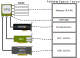
\includegraphics{bus-enumeration}
    \caption[Devices are part of the same address space as the \glsfmtshort{cpu} and system memory]
    {Device memory regions (\glsxtrshortpl{bar}) are part of the same address space as \glsxtrshort{cpu} and system memory, allowing
    the \gls{cpu} to read from and write to device memory the same way it would access \glsxtrshort{ram}. Devices can similarly use \gls{dma} to read from and write to \glsxtrshort{ram}.}
    \label{fig:bus-enumeration}
\end{figure}
The defining feature of \gls{pcie}~\cite{spec:PCIe} is that devices are mapped into the same address space as the \gls{cpu} and \gls{ram}, as seen in \cref{fig:bus-enumeration}.
%
This allows a \gls{cpu} to read from and write to device memory in the same manner it would access \gls{ram}, also known as \gls{mmio}.
%
Likewise, devices capable of \gls{dma} may read from and write to \gls{ram} directly.
%
\Gls{pcie} also uses \gls{msi}, allowing devices to raise interrupts by writing to an address reserved by the \gls{cpu} instead of requiring dedicated interrupt lines.



This mapping to the same address space occurs when a system enumerates the \gls{pcie} bus and accesses the \gls{cfgspace} of each device.
%
A \gls{cfgspace} contains a description of the capabilities of a device, such as its memory regions.
%
The system will reserve a memory address range for each of these device memory regions, and by writing the start address of these regions to the device's \glspl{bar}, a device is made aware of the address space mapping.
%
Therefore, the term ``\gls{bar}'' is used interchangeably for a region of device memory.
%
Addresses reserved by the system for interrupts are also written to the device's \gls{cfgspace}.



\begin{figure}
    \centering
    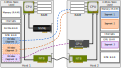
\includegraphics[width=.99\textwidth]{ntb-example}
    \caption[Two computer systems connected using \glsfmtshortpl{ntb}, and the \glsfmtshortpl{ntb} translate between the two different address domains]
    {Two computer systems connected together using \glspl{ntb} and external cables. Host~1 has mapped segments of Host~2's memory through its local \gls{ntb}, providing Host~1 with ``windows'' into the remote system's address space. The \glspl{ntb} translate addresses between the two independent address spaces.}
    \label{fig:ntb-example}
\end{figure}



As depicted in \cref{fig:ntb-example}, it is possible to connect computer systems with different address spaces together over \gls{pcie} by using \glspl{ntb}.
%
\Glspl{ntb} can be embedded as a \gls{cpu} feature~\cite{whitepaper:Sullivan2010,url:LinuxNTB-AMD}, but are more commonly implemented in \gls{pcie} switch chips~\cite{whitepaper:PLX,pex8733}.
%
By using such \gls{ntb}-capable switch chips to implement peripheral devices, independent computer systems can connect with plug-in host adapter cards and external cables.
%
To the system, the \gls{ntb} appears as a normal \gls{pcie} device\footnote{The \gls{pcie} terminology for individual \glspl{devicefunction} is ``\glspl{ep}''. We use the terms ``device'' and ``\gls{function}'' as synonyms for a \gls{pcie} \gls{ep} throughout this dissertation.} with one or more \glspl{bar} that are reserved and mapped during the enumeration process.
%
However, rather than being backed by device registers or device memory, the \gls{ntb} instead forwards reads and writes to its \glspl{bar} from one side of the \gls{ntb} to the other, translating memory addresses in the process.
%
The \gls{ntb} uses a \gls{lut} for address translation, which can be configured dynamically during run-time.
%
By using different base offsets in this \gls{lut}, it is possible to configure several memory-mappings (or ``windows'') into the address space of a remote system.
%
\Cref{fig:ntb-example} illustrates how arbitrary memory addresses on the remote system can be mapped, allowing the local \gls{cpu} to access remote memory as if it was local device memory.
%
Although address translation between the different address spaces is very fast since the \gls{lut} is implemented in \gls{ntb} hardware, the number of \gls{ntb} windows is limited by the maximum number of table entries.



Since device memory on a remote system is part of the same address space as system memory, we can use an \gls{ntb} to map memory of a remote device.
%
We show this in \cref{fig:ntb-example}, where Segment~3 is allocated in \gls{gpu} memory rather than system~\gls{ram}, but still mapped for the \gls{cpu} of Host~1's similarly to the other segments.
%
By mapping all \glspl{bar} of a remote device for a local \gls{cpu}, it would be possible to perform memory operations on the remote device, such as reading from or writing to device registers.
%
Moreover, device~\gls{dma} is not limited to reading and writing to system \gls{ram}, but can also be used to access memory on other devices in the same address space.
%
This is known as ``\gls{p2p}'' in \gls{pcie}, and provides us with an opportunity as it becomes possible for a device to read and write directly across an \gls{ntb}.
%
We can use this to map memory resources for a device, be it \gls{ram} or memory of other devices. 
%
Furthermore, because \gls{pcie} uses \gls{msi}, it is even possible to map interrupt addresses through an \gls{ntb}, as they too are mappable.



However, although \glspl{ntb} provide the fundamental memory mapping capabilities that can facilitate the use of remote devices, the challenge is to avoid requiring device drivers to be aware of remote-side address spaces.
%
As touched upon in \cref{sec:motivation}, this is desirable in order to use existing device driver implementations.
%
In order for a device driver running on a local~machine to use a remote~device, we must make sure that the driver uses addresses that is mapped through both the local and remote \glspl{ntb}.
%
For instance, when the device driver attempts to access device~\glspl{bar}, we must make sure that the driver uses memory addresses that are mapped through the local, or \gls{cpu}-side, \gls{ntb} without the driver or device being aware of this.
%
Conversely, when the device driver attempts to initiate \gls{dma} transfers or configures an interrupt vector address, we must find a way to transparently inject memory addresses that are mapped through the remote, or device-side, \gls{ntb}.



\Gls{dma} is particularly challenging in this context.
%
Device drivers may assume that any local memory address can be reached by the device, but the \gls{ntb} only provide \emph{windows} into a remote address space.
%
It is generally not possible to predict in advance which memory addresses a device driver may use, yet memory must be mapped through the \gls{ntb} before the driver initiates \gls{dma} transfers.
%
Deferring the action of setting up these maps until the device driver initiates \gls{dma}, or some other time when the specific addresses of \gls{dma} buffers may be known, is not viable;
%
synchronizing with the remote system at this time will introduce communication overhead in the performance-critical path.
%
A naive solution is to map the entire system memory, but this workaround does not scale very well since it would require the \gls{ntb}~\glspl{bar} to be \emph{as large} as the size of \gls{ram}.
%
Not only will the memory requirements increase for every machine added to the cluster, but the number of maps supported by the \gls{ntb} is limited by the size of its \gls{lut}.




One possibility is to use virtualization to mitigate the complexity of managing different address spaces.
%
The fact that devices are on the other side of an \gls{ntb} could be hidden for device drivers by distributing devices to \gls{vm} \glspl{guest} instead of physical \lgls{host}{host~machines}.
%
The \gls{hypervisor} on a \lgls{host}{host~machine} can be modified to assist setting up necessary \gls{ntb} (and \gls{iommu}) mappings to the respective device memory and \gls{vm} memory.
%
This would make it possible to \gls{passthrough} a remote device to a \gls{vm} \gls{guest} running on a local \lgls{host}{host~machine}.
%
However, requiring that compute tasks run in \glspl{vm} limits the generality of a solution.
%
Virtualization is not necessarily appropriate in all circumstances, as it may add additional system load because \gls{cpu} cycles are spent on \lgls{host}{hosting} the virtualized environment.
%
A more general mechanism is needed for abstracting away the complexity of dealing with a remote-side address space and allowing device drivers to remain agnostic about different address spaces.
%
%%% TODO FIXME NOTE: Pål wanted to end this paragraph with "this is how we do it" or "we support X or Y" or something like this



For more details on \glspl{ntb} and \gls{pcie}, particularly how memory transactions are routed, please refer to \paperref{tocs:pcie}. See also \paperref{cc:pcie}.

\section{Implementation}\label{sec:impl}
In our framework, computer systems act as \emph{``\glspl{borrower}''} and \emph{``\glspl{lender}''}.
%
A \gls{lender} is a computer system that registers one or more of its internal \gls{pcie} devices with SmartIO, allowing the devices to be distributed to and used by remote machines.
%
A \gls{borrower} is a system that is currently using such a device. 
%
While a device only has one \gls{lender}, namely the computer system where it is physically installed, there can be several \glspl{borrower} using it simultaneously.
%
SmartIO also makes it possible for a system to act as both \gls{lender} and \gls{borrower} at the same time, lending out its own local devices and simultaneously borrowing remote devices from other machines.
%
All machines in the cluster~network may contribute their own local resources and access remote resources.


Since remote devices and memory resources are accessed over native \gls{pcie}, they can be shared and used by remote machines with very low latency and extremely low computing overheads.
%
The hard separation between local and remote is blurred, with regard to both functionality and performance.
%
Furthermore, as we rely on standard \gls{pcie}, the implementation complexity of SmartIO lies in software.
%
SmartIO can be implemented for existing computer systems that are connected with \glspl{ntb} in any network topology, using either on-board \gls{pcie} switch chips with \gls{ntb} capabilities or \glspl{ntb} implemented as plug-in adapter cards.
%
For more details on \glspl{ntb} and \gls{pcie} in general, please refer to \paperref{tocs:pcie}.


\begin{figure}
    \centering
    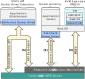
\includegraphics{software-architecture}
    \caption[SmartIO facilitates access to a remote resource via different interfaces]
    {SmartIO facilitates access to remote resources via different interfaces.
    %
    These interfaces present an abstraction layer to application software and device drivers, providing a logical decoupling of devices and which physical machines they are installed in.}
    \label{fig:architecture}
\end{figure}


Unlike other solutions for distributed \gls{io}, SmartIO combines traditional \gls{io} with distributed shared-memory functionality in a seamless manner.
%
Thus, sharing is supported at multiple abstraction levels:
%
devices may be distributed to physical \glspl{hostmachine} and to \glspl{vm} alike.
%
Additionally, SmartIO provides software facilities for \gls{disaggregating} devices and memory resources, allowing device drivers to be implemented as part of distributed cluster applications in \gls{userspace}.
%
There may be several separate software processes on the same machine using a device, or running on different hosts altogether.
%
\Cref{fig:architecture} illustrates the different components of the SmartIO framework, and how they fit together:
\begin{enumerate}
    \item \textbf{Low-level \gls{ntb} driver}:
        %
        our SmartIO framework is built on top of the \gls{ntb} cluster interconnection solution from Dolphin.
        %
        The low-level \gls{ntb} driver provides \gls{pcie} networking functionality as well as basic shared-memory functionality which  SmartIO builds on.
        %
        Moreover, application software may use the \gls{sisciapi} to implement shared-memory communication.

    \item \textbf{Address resolution mechanism}: 
        SmartIO provides functionality for 
        

        %
        this makes it possible to abstracting away the physical location of devices and memory segments,~i.e., which machines they are installed in.

        %
        functionality for transparently translating \gls{io} addresses between th different address spaces

        and is able to abstract away the location of devices and memory segments,~i.e., which machines they are installed in.

        (or device-side) addresses.
        %
        With this abstraction, SmartIO facilitates the use of remote resources (both memory and devices) without requiring the user to be aware of the underlying, physical \gls{pcie} topology or the internal \gls{io} address space layout of remote machines.
        %
        Furthermore, this mechanism is also able to support mapping 

    \item \textbf{Device Lending}:

    \item \textbf{\gls{mdev}}:

    \item \textbf{\gls{sisciapi} extension}:
\end{enumerate}






%\paperref{tocs}{pcie-addr}



%%
%Also unlike existing \gls{pcie}-based solutions, SmartIO is fully distributed and avoids dedicated servers.
%All machines in the cluster can contribute their own local resources and access remote resources, even at the same time.
%%
%Finally, by using \gls{pcie} shared memory techniques, SmartIO is able to abstract away the physical location of devices and memory resources. 
%Memory addresses are translated between different address domains by SmartIO in a manner that is transparent to application software, device drivers, and even the \gls{os}.
%This makes it possible to provide optimizations based on resource locality and minimizing data movement, without requiring the user to be aware of the underlying PCIe topology.
%\section{General idea}\label{sec:idea}
%High level explanation of borrowers and lenders here.
%Software architecture figure (showing the different components here)

\subsection{Device Lending}
\begin{itemize}
    \item explain shadow device
    \item intercept configuration cycles
    \item hooking DMA api for setting up DMA windows
    \item IOMMU discussion
\end{itemize}

\subsection{MDEV}
\begin{itemize}
    \item \textbf{very} brief: what is passthrough/VFIO
    \item what MDEV gives us
    \item how to map VM memory for device
    \item relaying interrupts
\end{itemize}

\subsection{API extension}
\begin{itemize}
    \item why do we need API? (disaggregation in software + shared memory networking)
    \item short explanation of SISCI
    \item what functions did we add to SISCI?
\end{itemize}

\subsection{Support for multiple lenders}
\begin{itemize}
    \item peer-to-peer device lending
    \item peer-to-peer vms
\end{itemize}


\subsection{NVMe driver}\label{sec:nvme}
\begin{itemize}
    \item why a prototype driver? demonstrate disaggregation in software
    \item why nvme? easy to parallelize because of queues
    \item driver implementation and queue sharing
    \item gpudirect + co-operation with device lending
\end{itemize}

%\section{Workload}\label{sec:eval}

\section{Performance measurements}\label{sec:eval}
Some selected performance graphs here, demonstrating zero-overhead :)

\section{Related work}\label{sec:rw}
should rw go in discussion and conclusion instead?
\begin{itemize}
    \item rdma stuff
    \item fabric partitioning: mr-iov, broadcom/microsemi chips with partitioning
    \item ladon (and other ntb stuff)
    \item disaggregation
\end{itemize}

\glspl{guest}

% RW first??
%An example of this is rCUDA, where multiple clients may run jobs on the same \gls{gpu} by relying ~\cite{Duato2010}
%\Gls{rdma}-based \gls{disaggregation} can even allow a single resource to be shared by several machines in the cluster at the same time. 
%
%However, since 
